\chapter*{More figures}
\addcontentsline{toc}{chapter}{More figures}

Some figures are referred to in the text but not placed directly under the text. These are included in this list. All figures are high resolution thus zooming in the PDF should be viable to get a clearer view.

%------------------------------------

\section*{Overview of training set}

\begin{figure}[H]
    \begin{center}
        \fbox{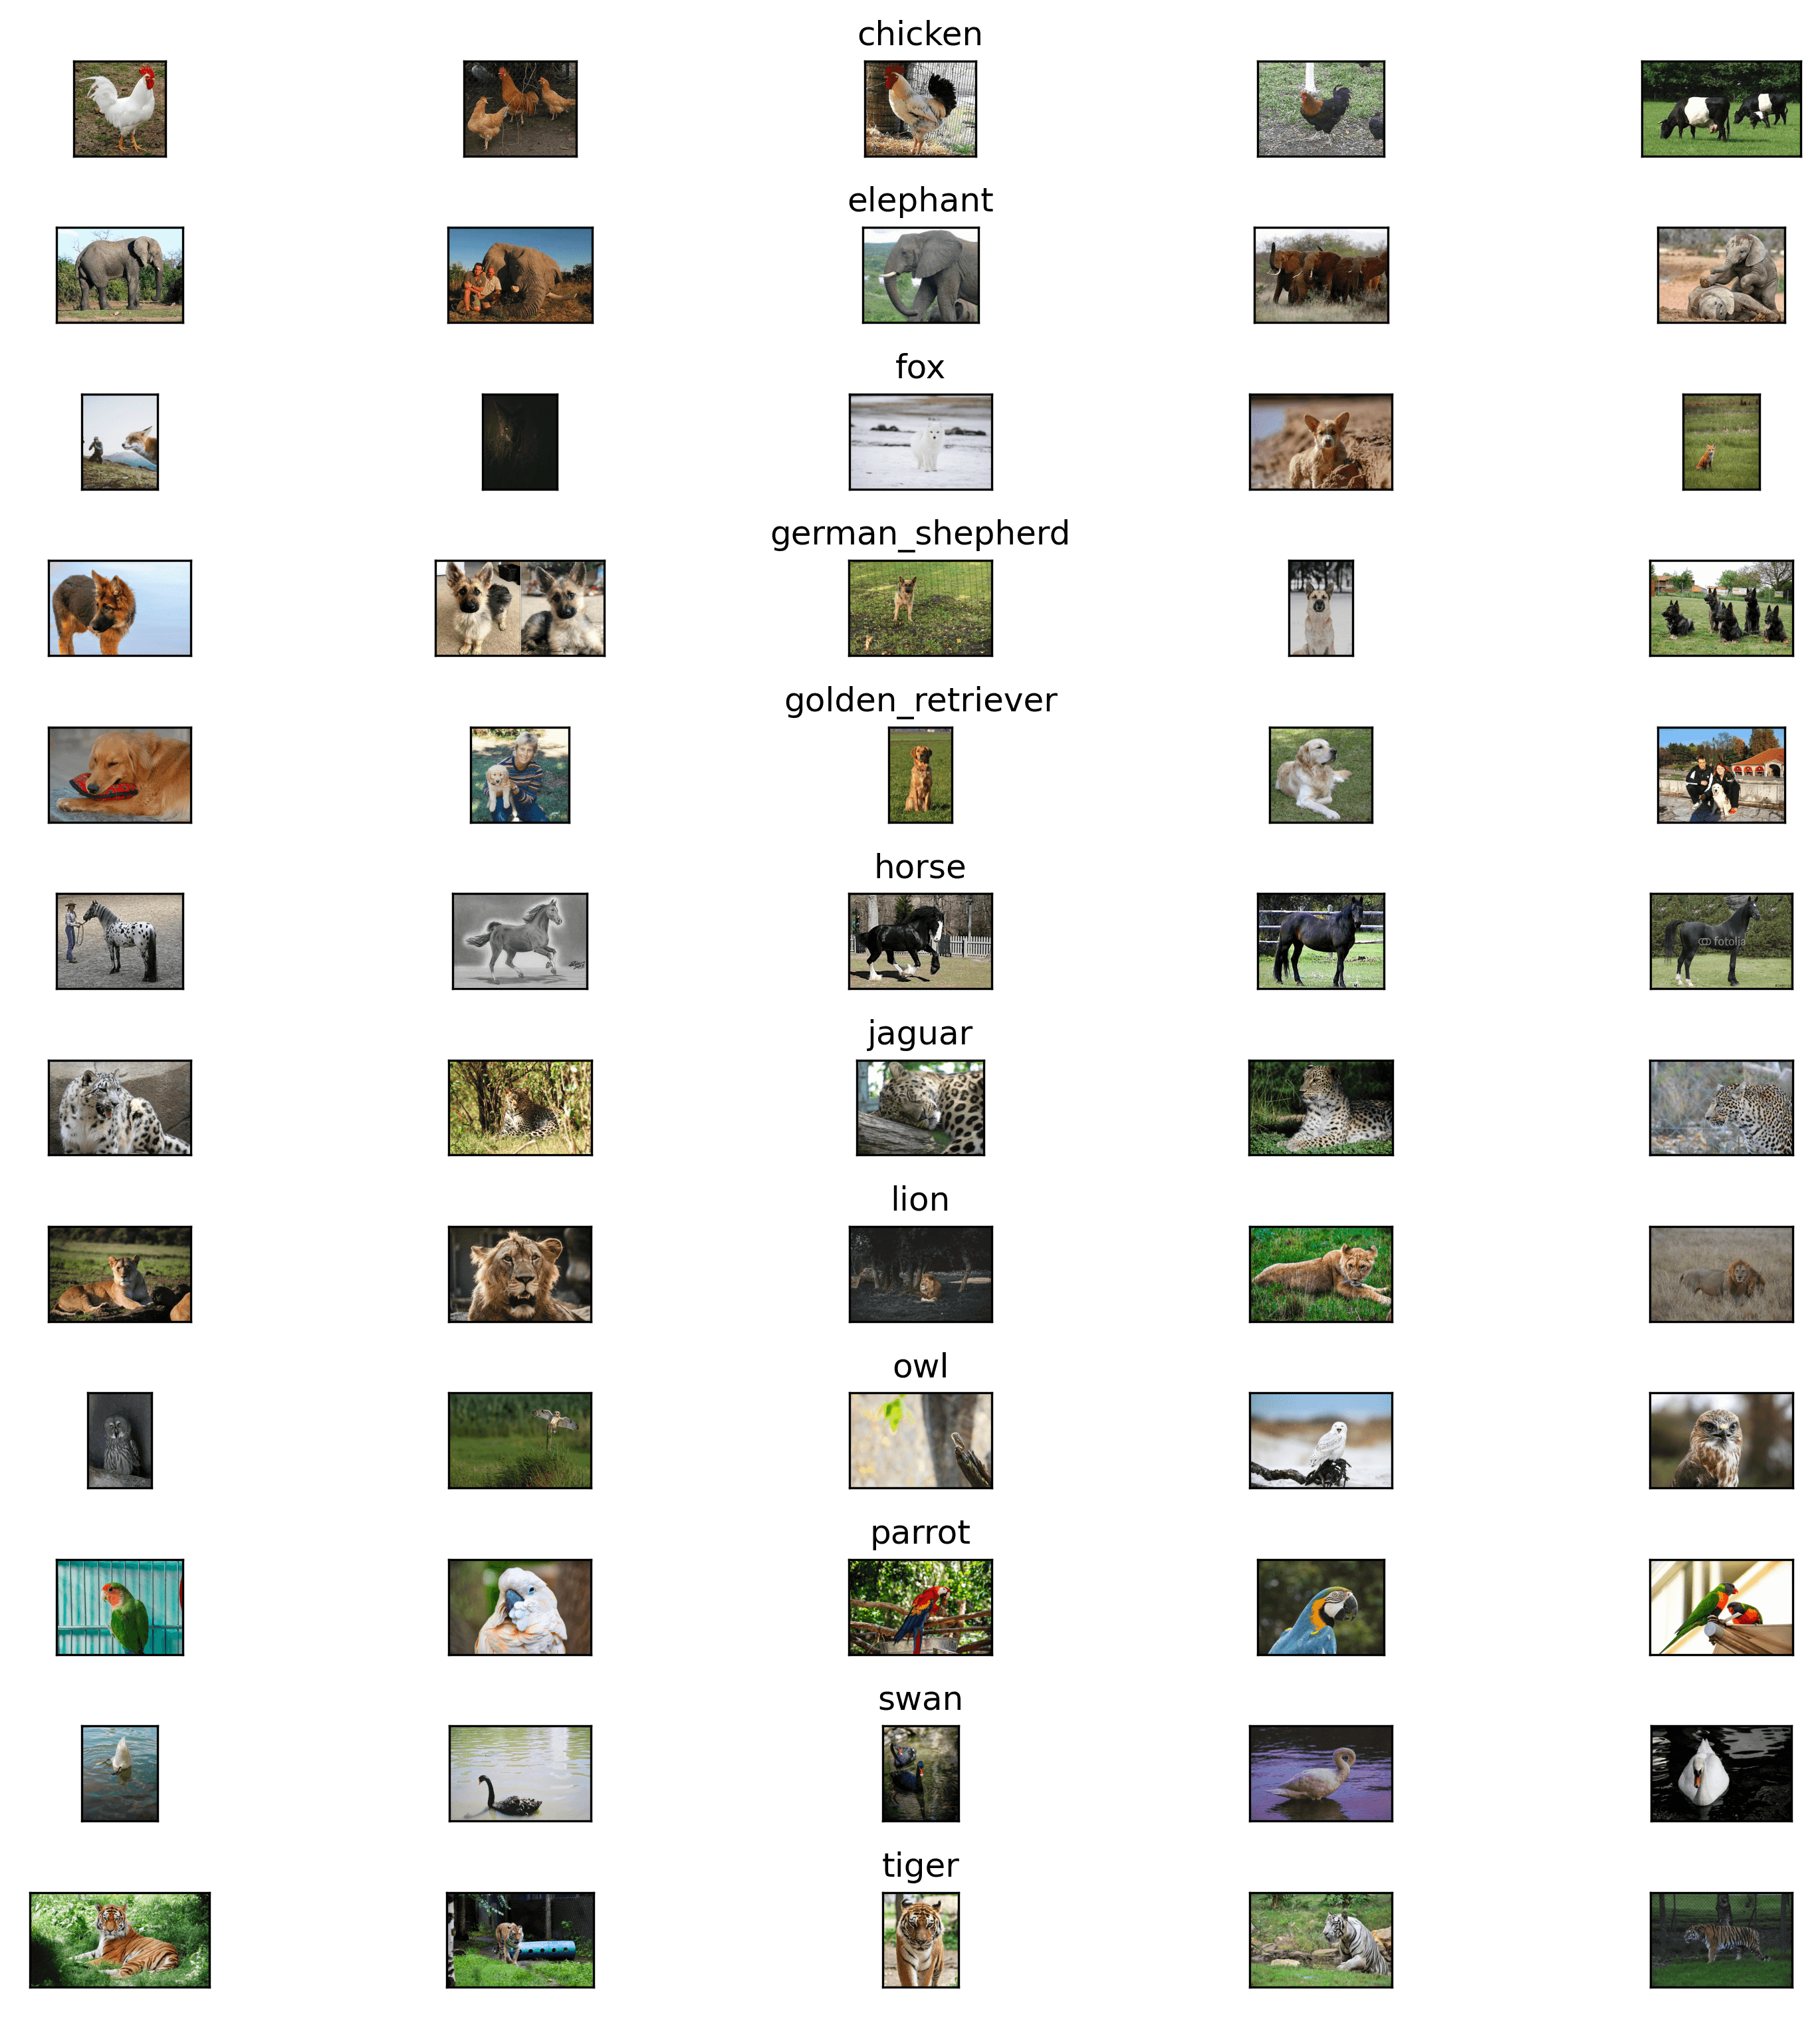
\includegraphics[width=0.6\linewidth]{images/1/1-data_analysis-labeled_data_overview.png}}
    \end{center}
    \captionsetup{width=0.65\linewidth}
    \captionsetup{justification=centering}
    \caption{An overview of the supplied data per class.}
    \label{fig:1-data_analysis-labeled_data_overview.png}
\end{figure}

%------------------------------------

\section*{Learning curves of the models}

\begin{figure}[H]
    \centering
    \fbox{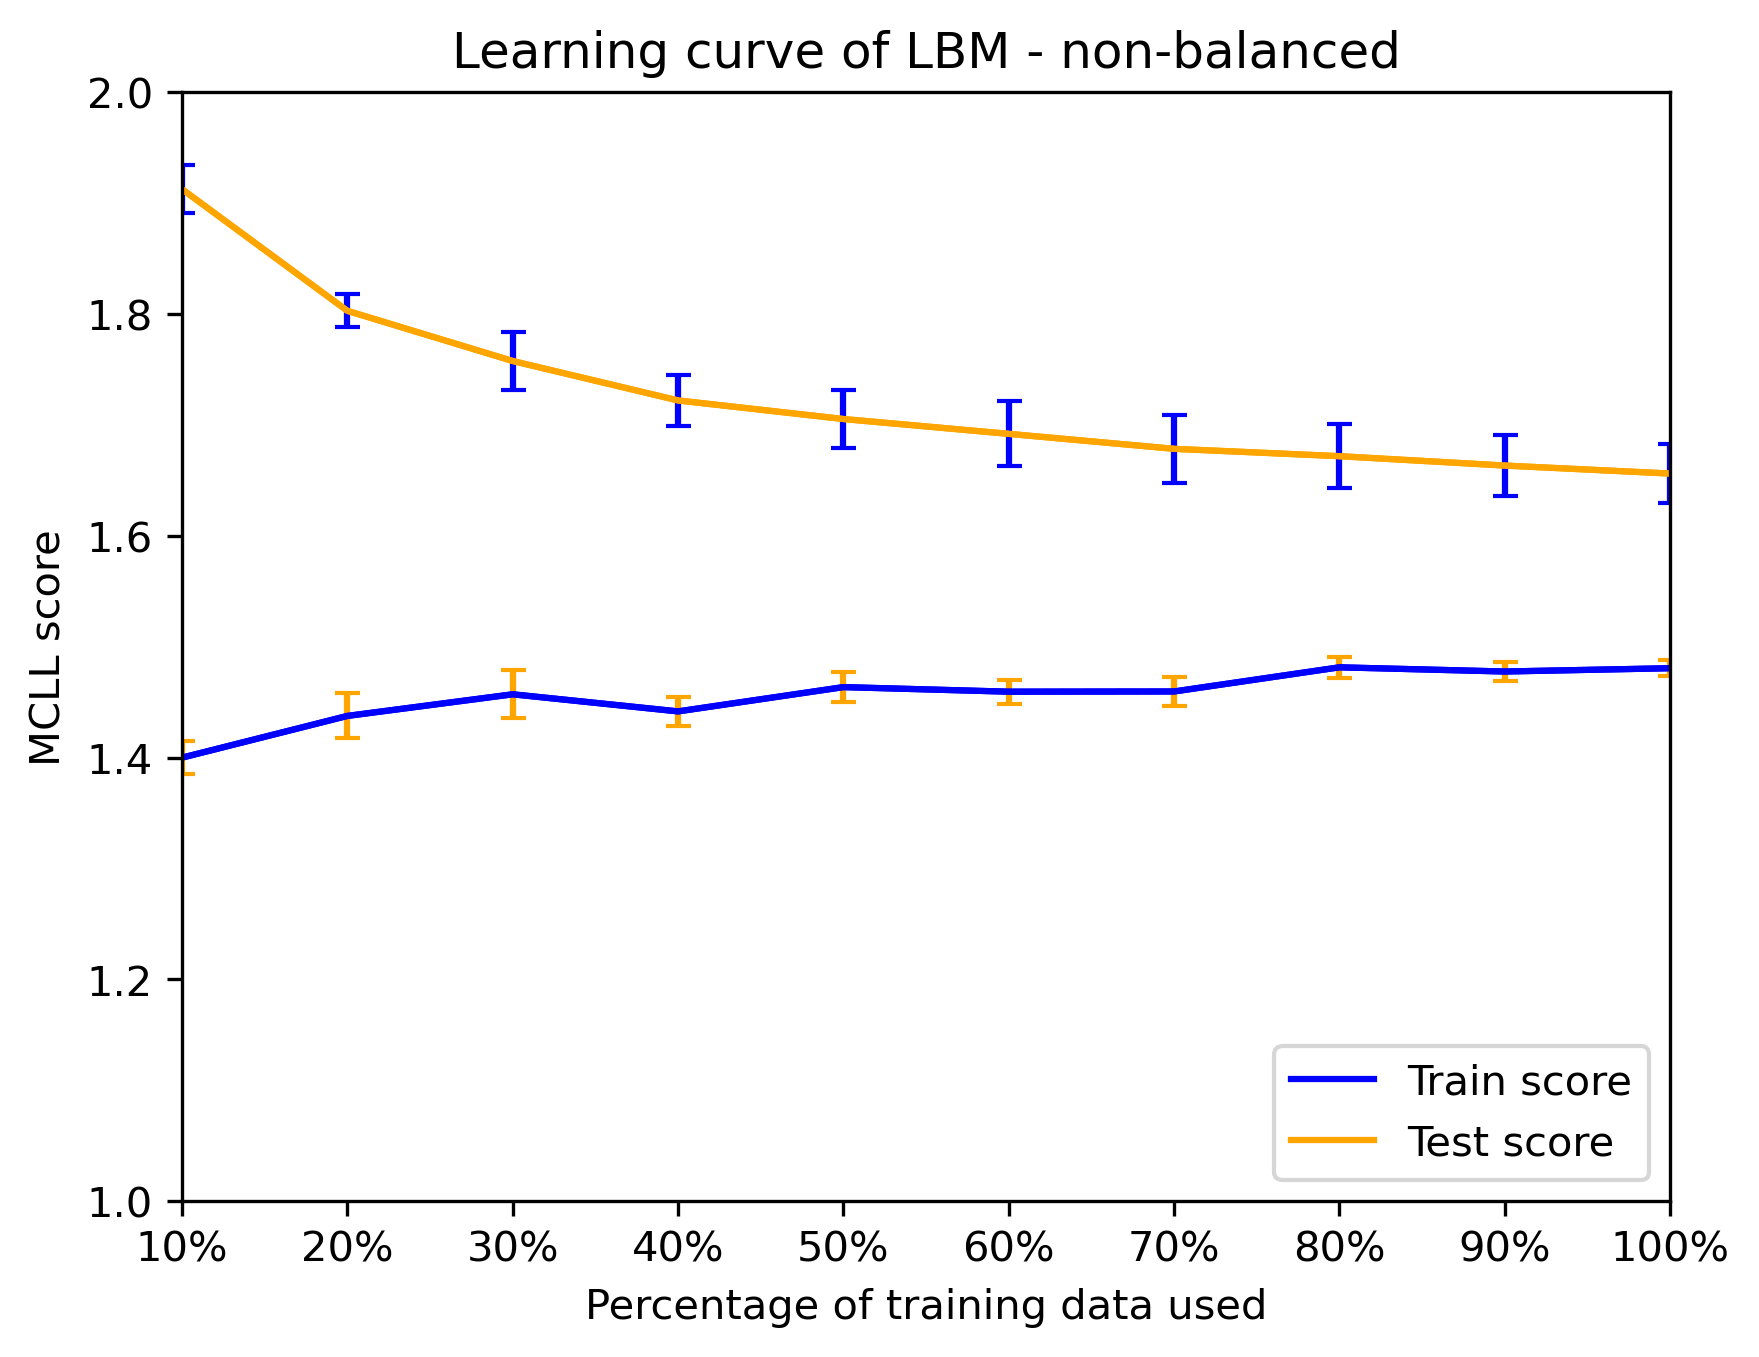
\includegraphics[width=0.65\linewidth]{images/MA/MA_LBM_learning_curve.png}}
    \captionsetup{width=0.6\linewidth}
    \captionsetup{justification=centering}
    \caption{Learning curve of the non-balanced linear baseline model.}
\end{figure}

\begin{figure}[H]
    \centering
    \fbox{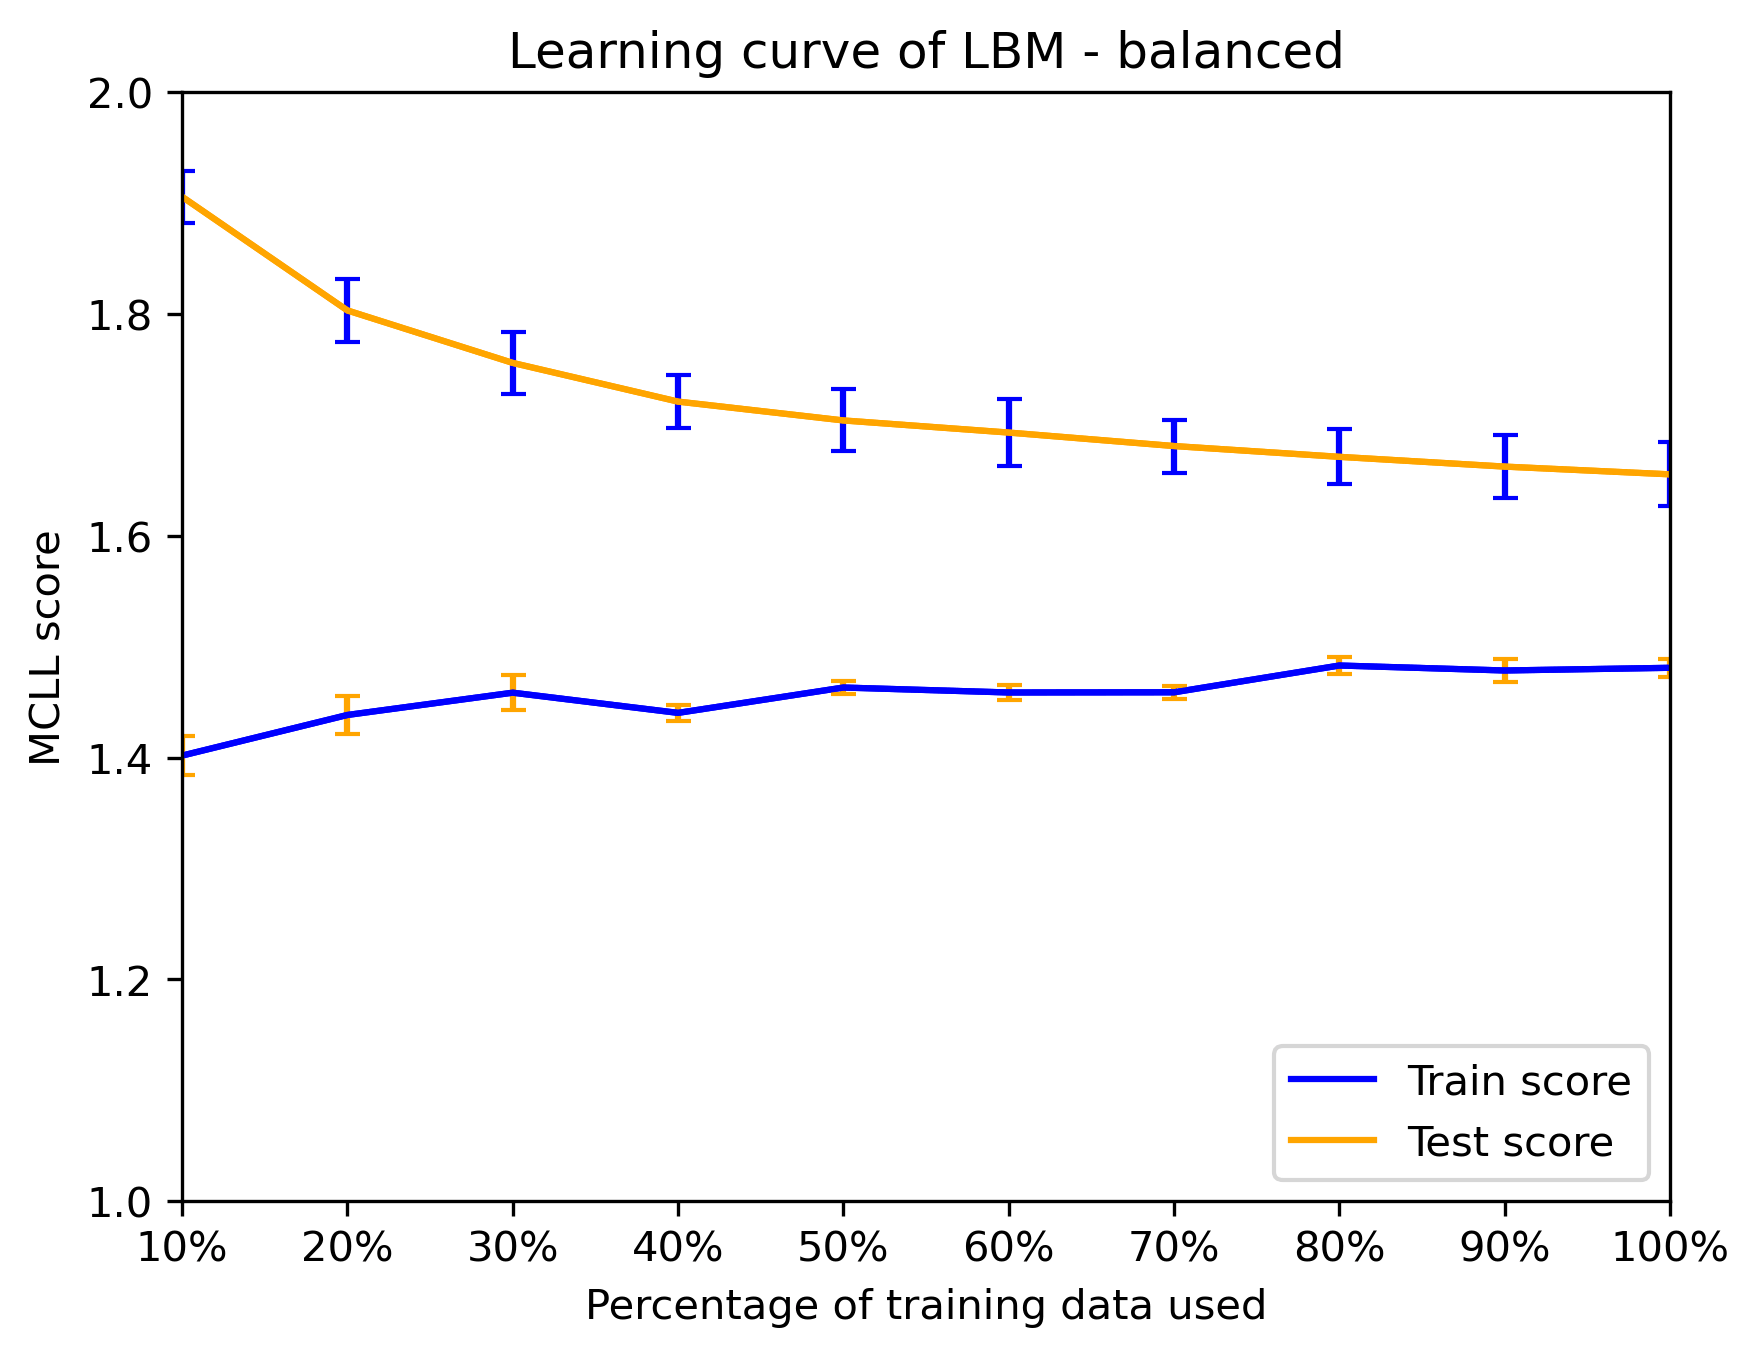
\includegraphics[width=0.65\linewidth]{images/MA/MA_LBM_learning_curve_balanced.png}}
    \captionsetup{width=0.6\linewidth}
    \captionsetup{justification=centering}
    \caption{Learning curve of the balanced linear baseline model.}
\end{figure}

\begin{figure}[H]
    \centering
    \fbox{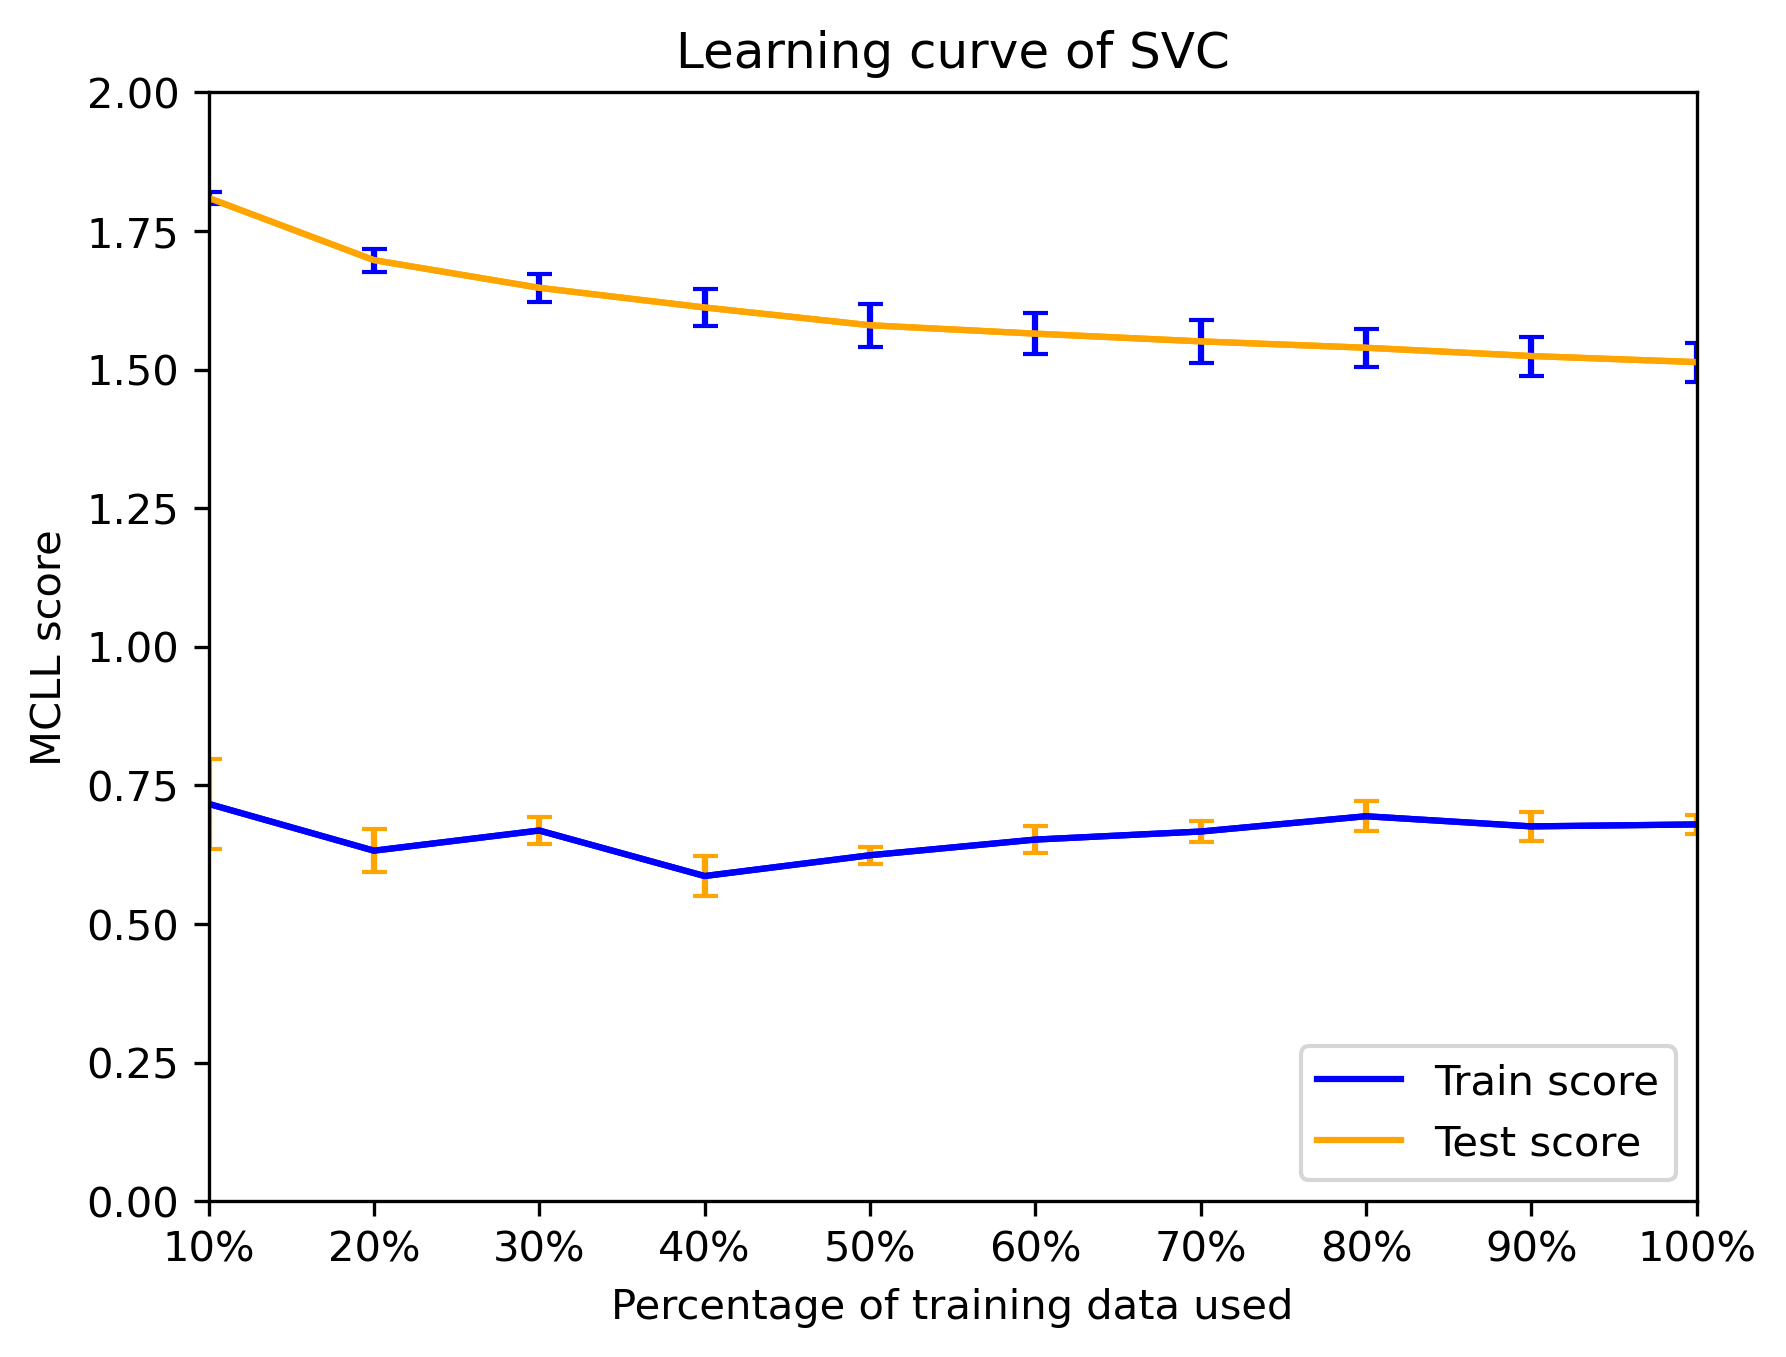
\includegraphics[width=0.75\linewidth]{images/MA/MA_SVC_learning_curve.png}}
    \captionsetup{width=0.7\linewidth}
    \captionsetup{justification=centering}
    \caption{Learning curve of the SVC model.}
\end{figure}

\begin{figure}[H]
    \centering
    \fbox{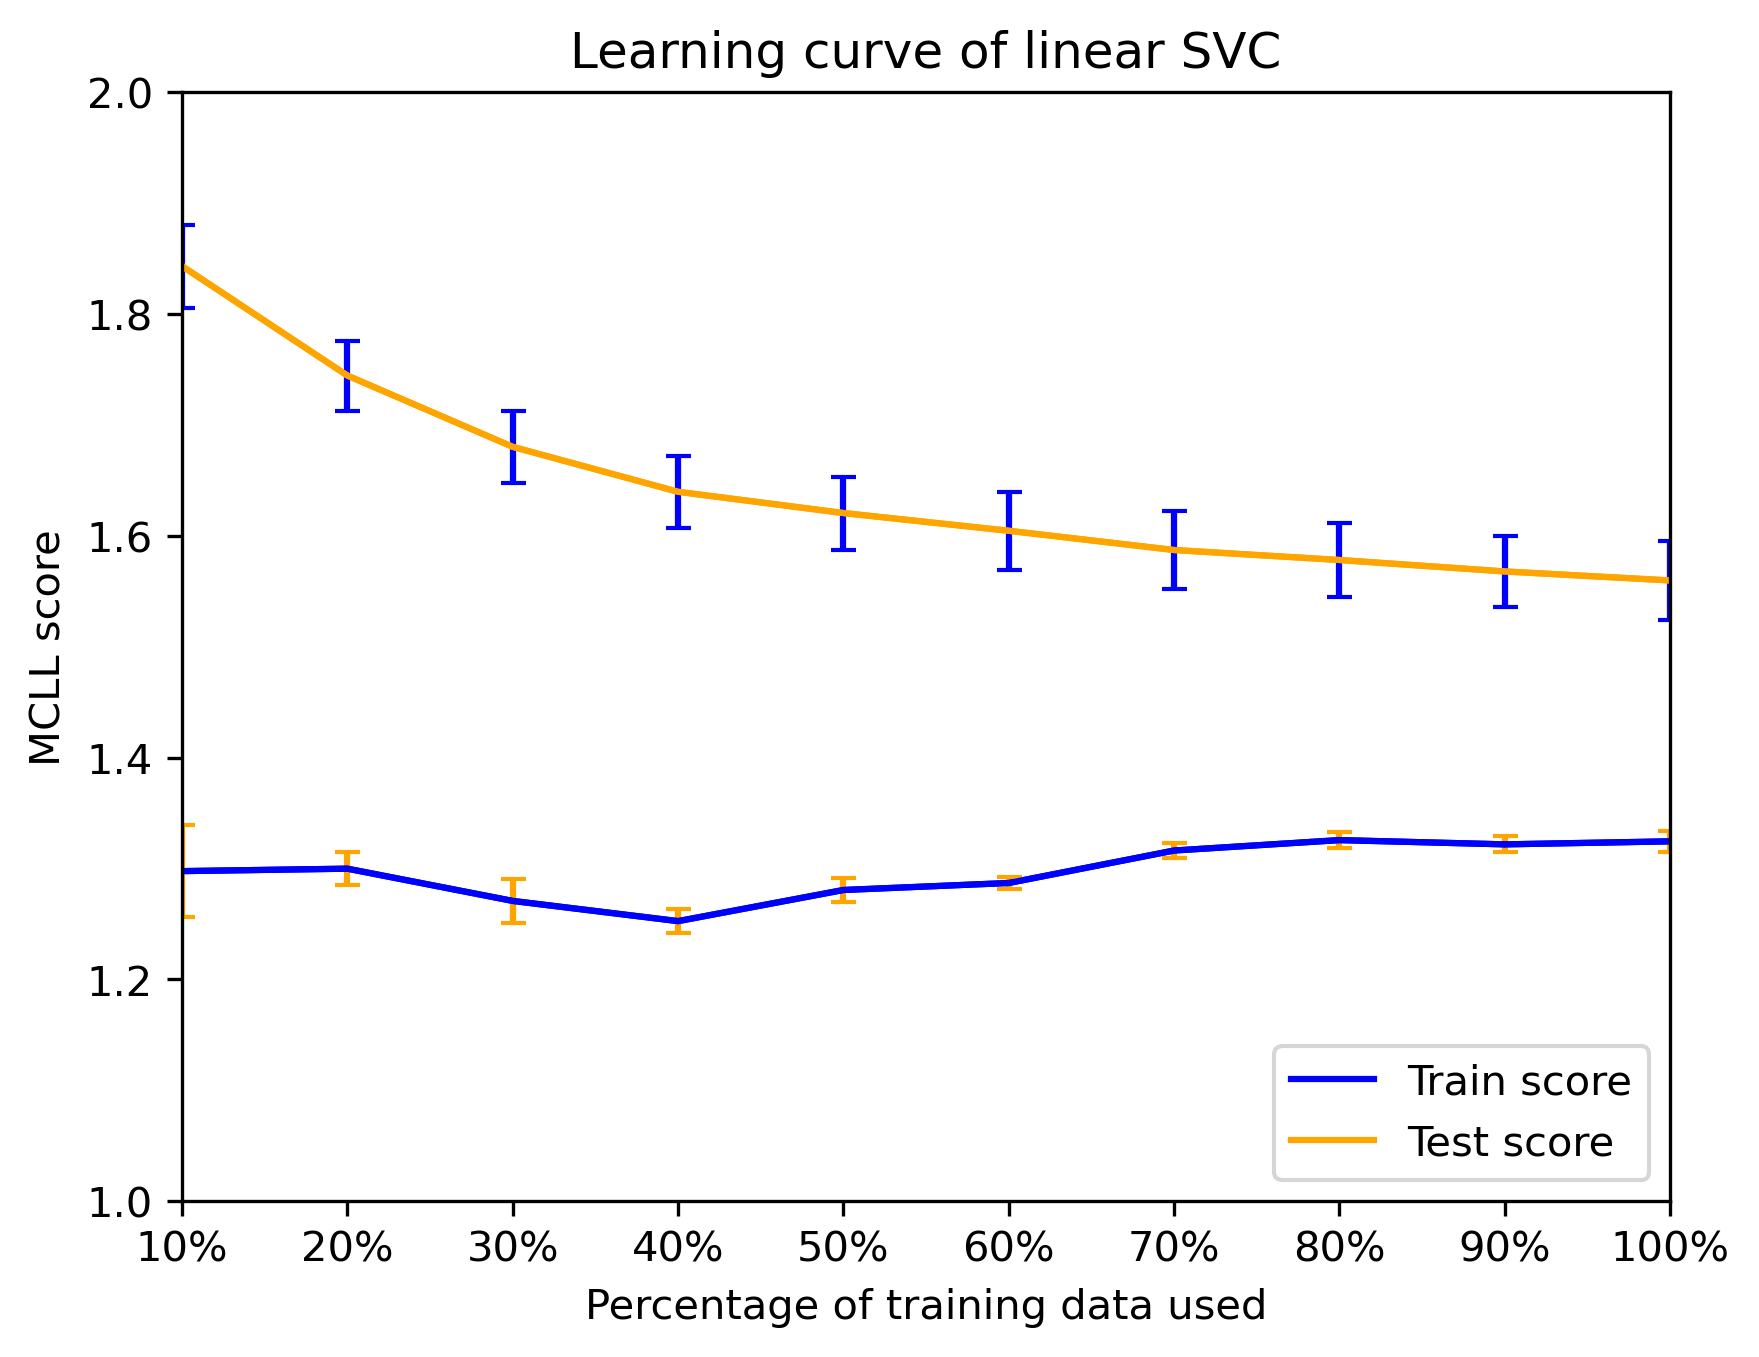
\includegraphics[width=0.75\linewidth]{images/MA/MA_linSVC_learning_curve.png}}
    \captionsetup{width=0.7\linewidth}
    \captionsetup{justification=centering}
    \caption{Learning curve of the linear SVC model.}
\end{figure}

%------------------------------------

\section*{Confusion matrix of linear SVC}

\begin{figure*}[ht]
    \centering
    \begin{subfigure}{.45\textwidth}
        \centering
        \fbox{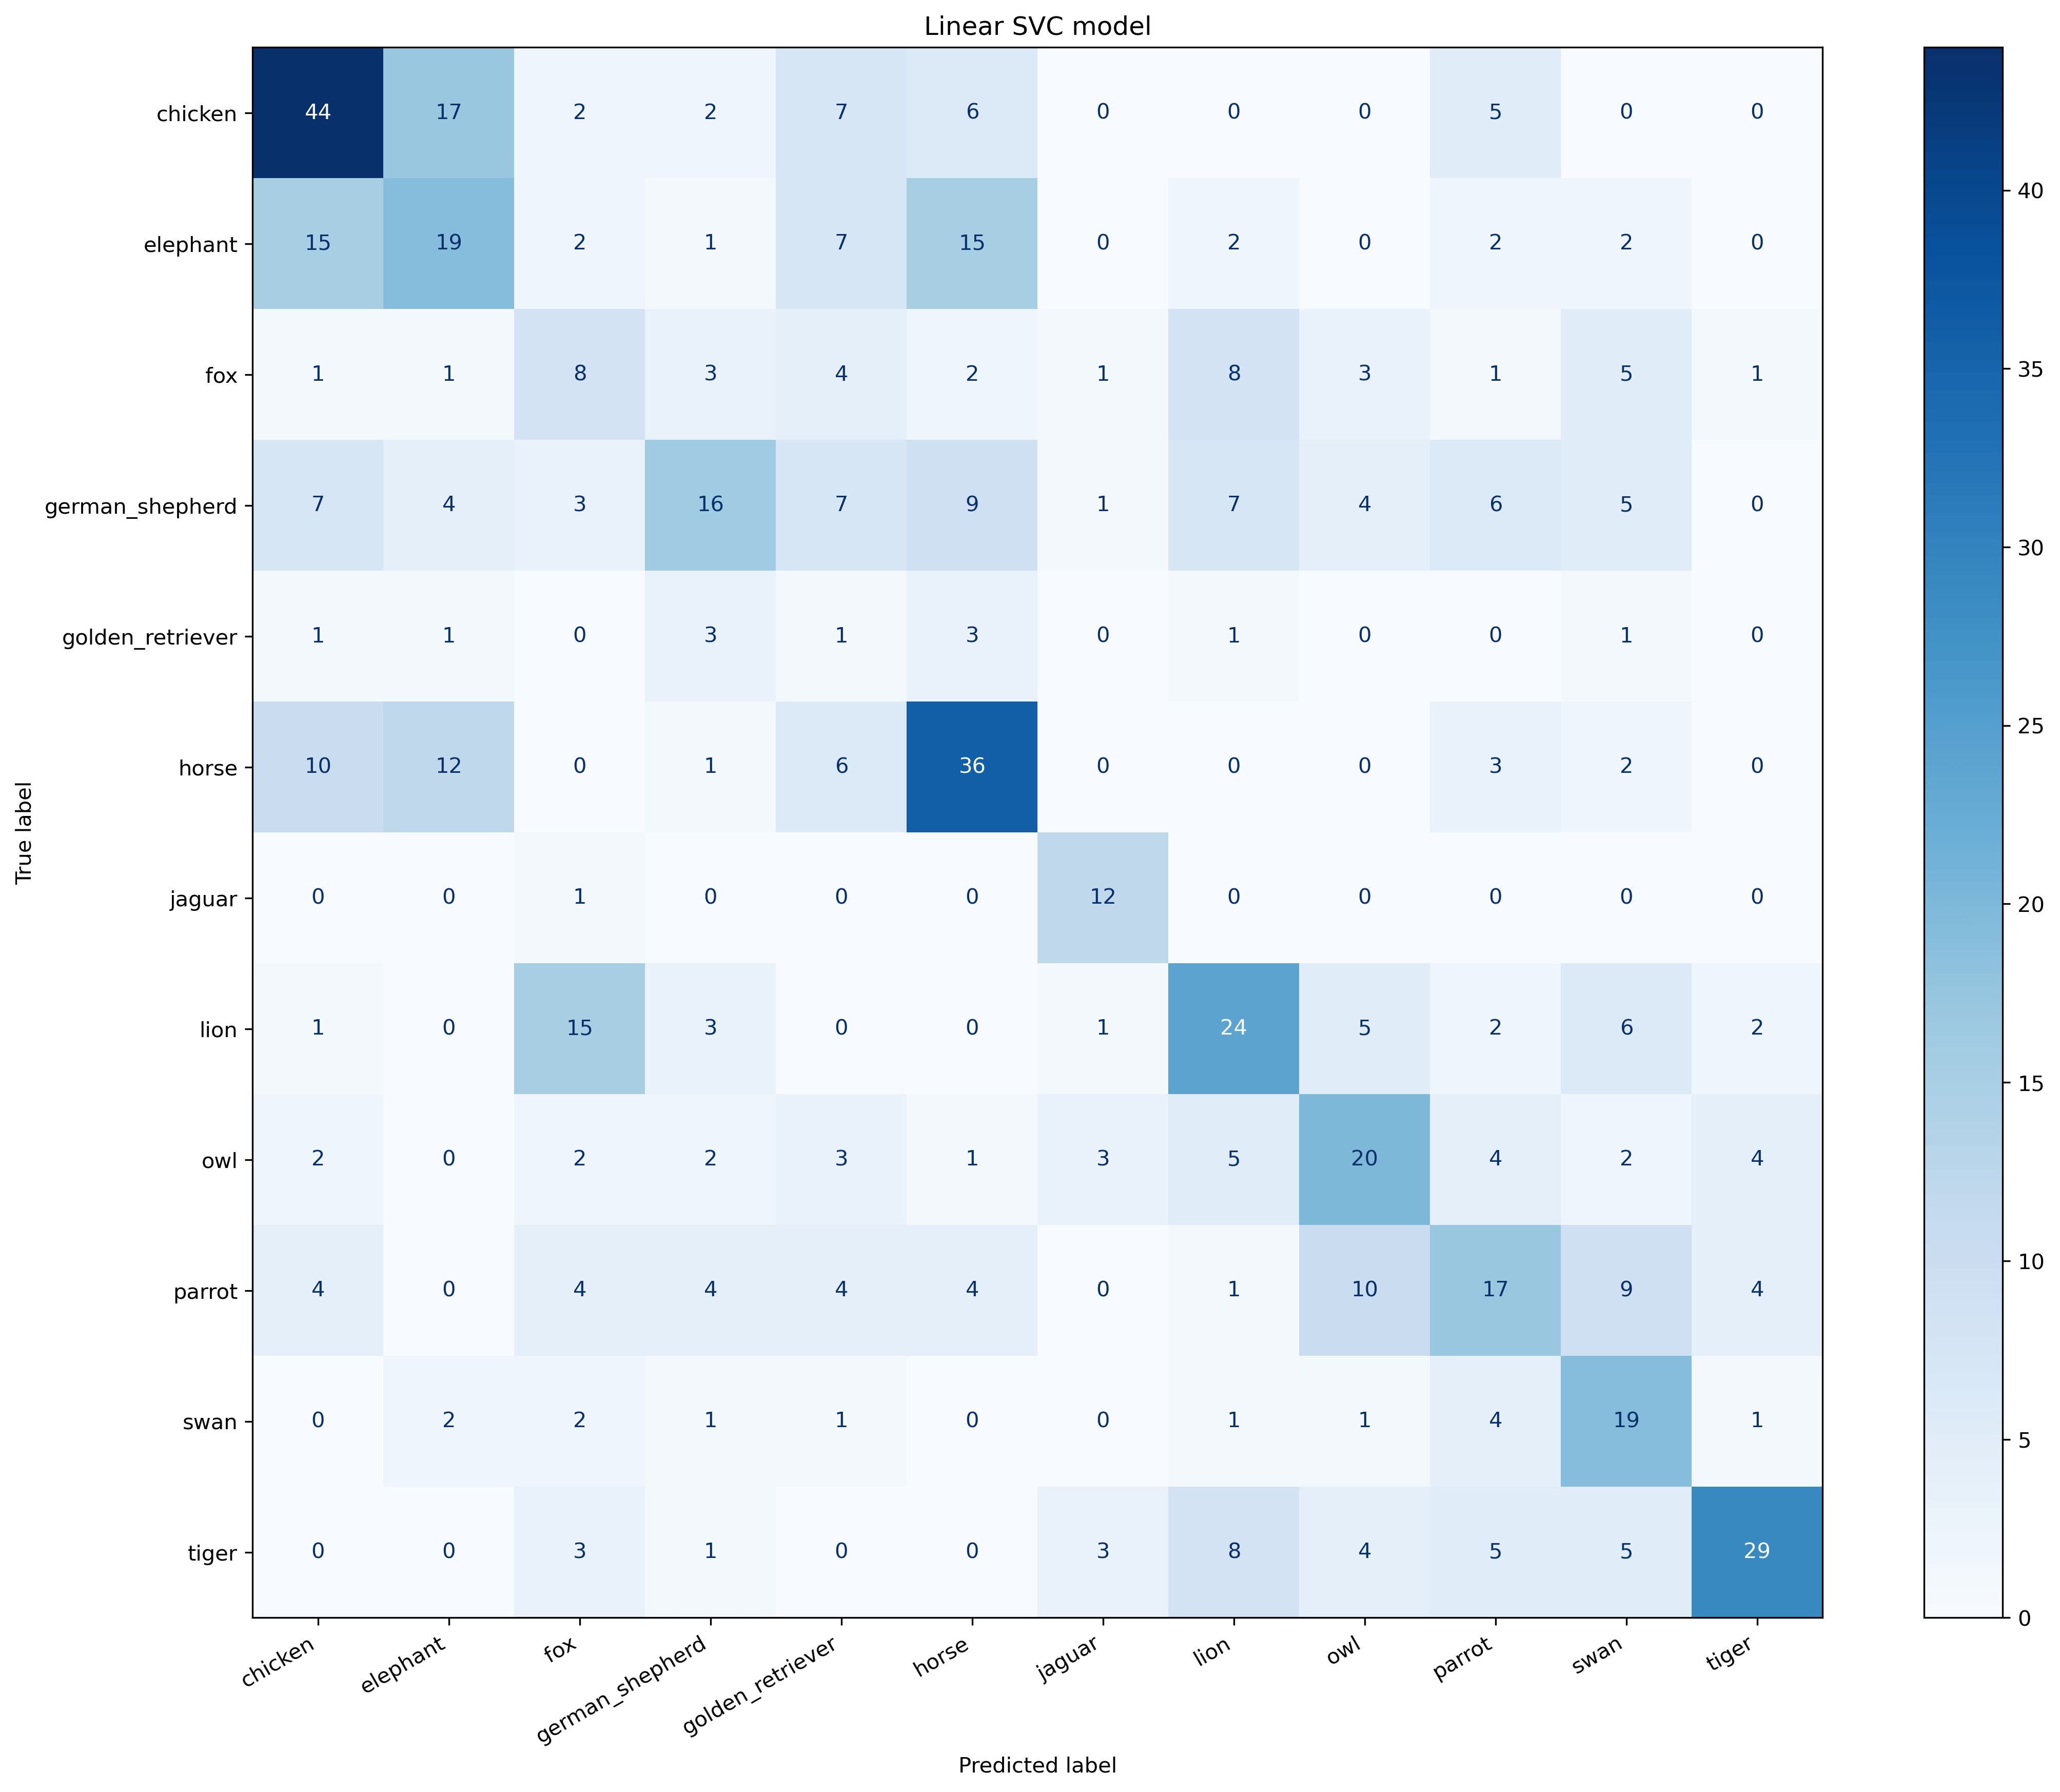
\includegraphics[width=\textwidth]{images/MA/MA_linSVC_non_normalised.png}}
        \captionsetup{width=0.9\linewidth}
        \captionsetup{justification=centering}
        \caption{Non normalised CM.}
    \end{subfigure}
    \hspace{1cm}
    \begin{subfigure}{.45\textwidth}
        \centering
        \fbox{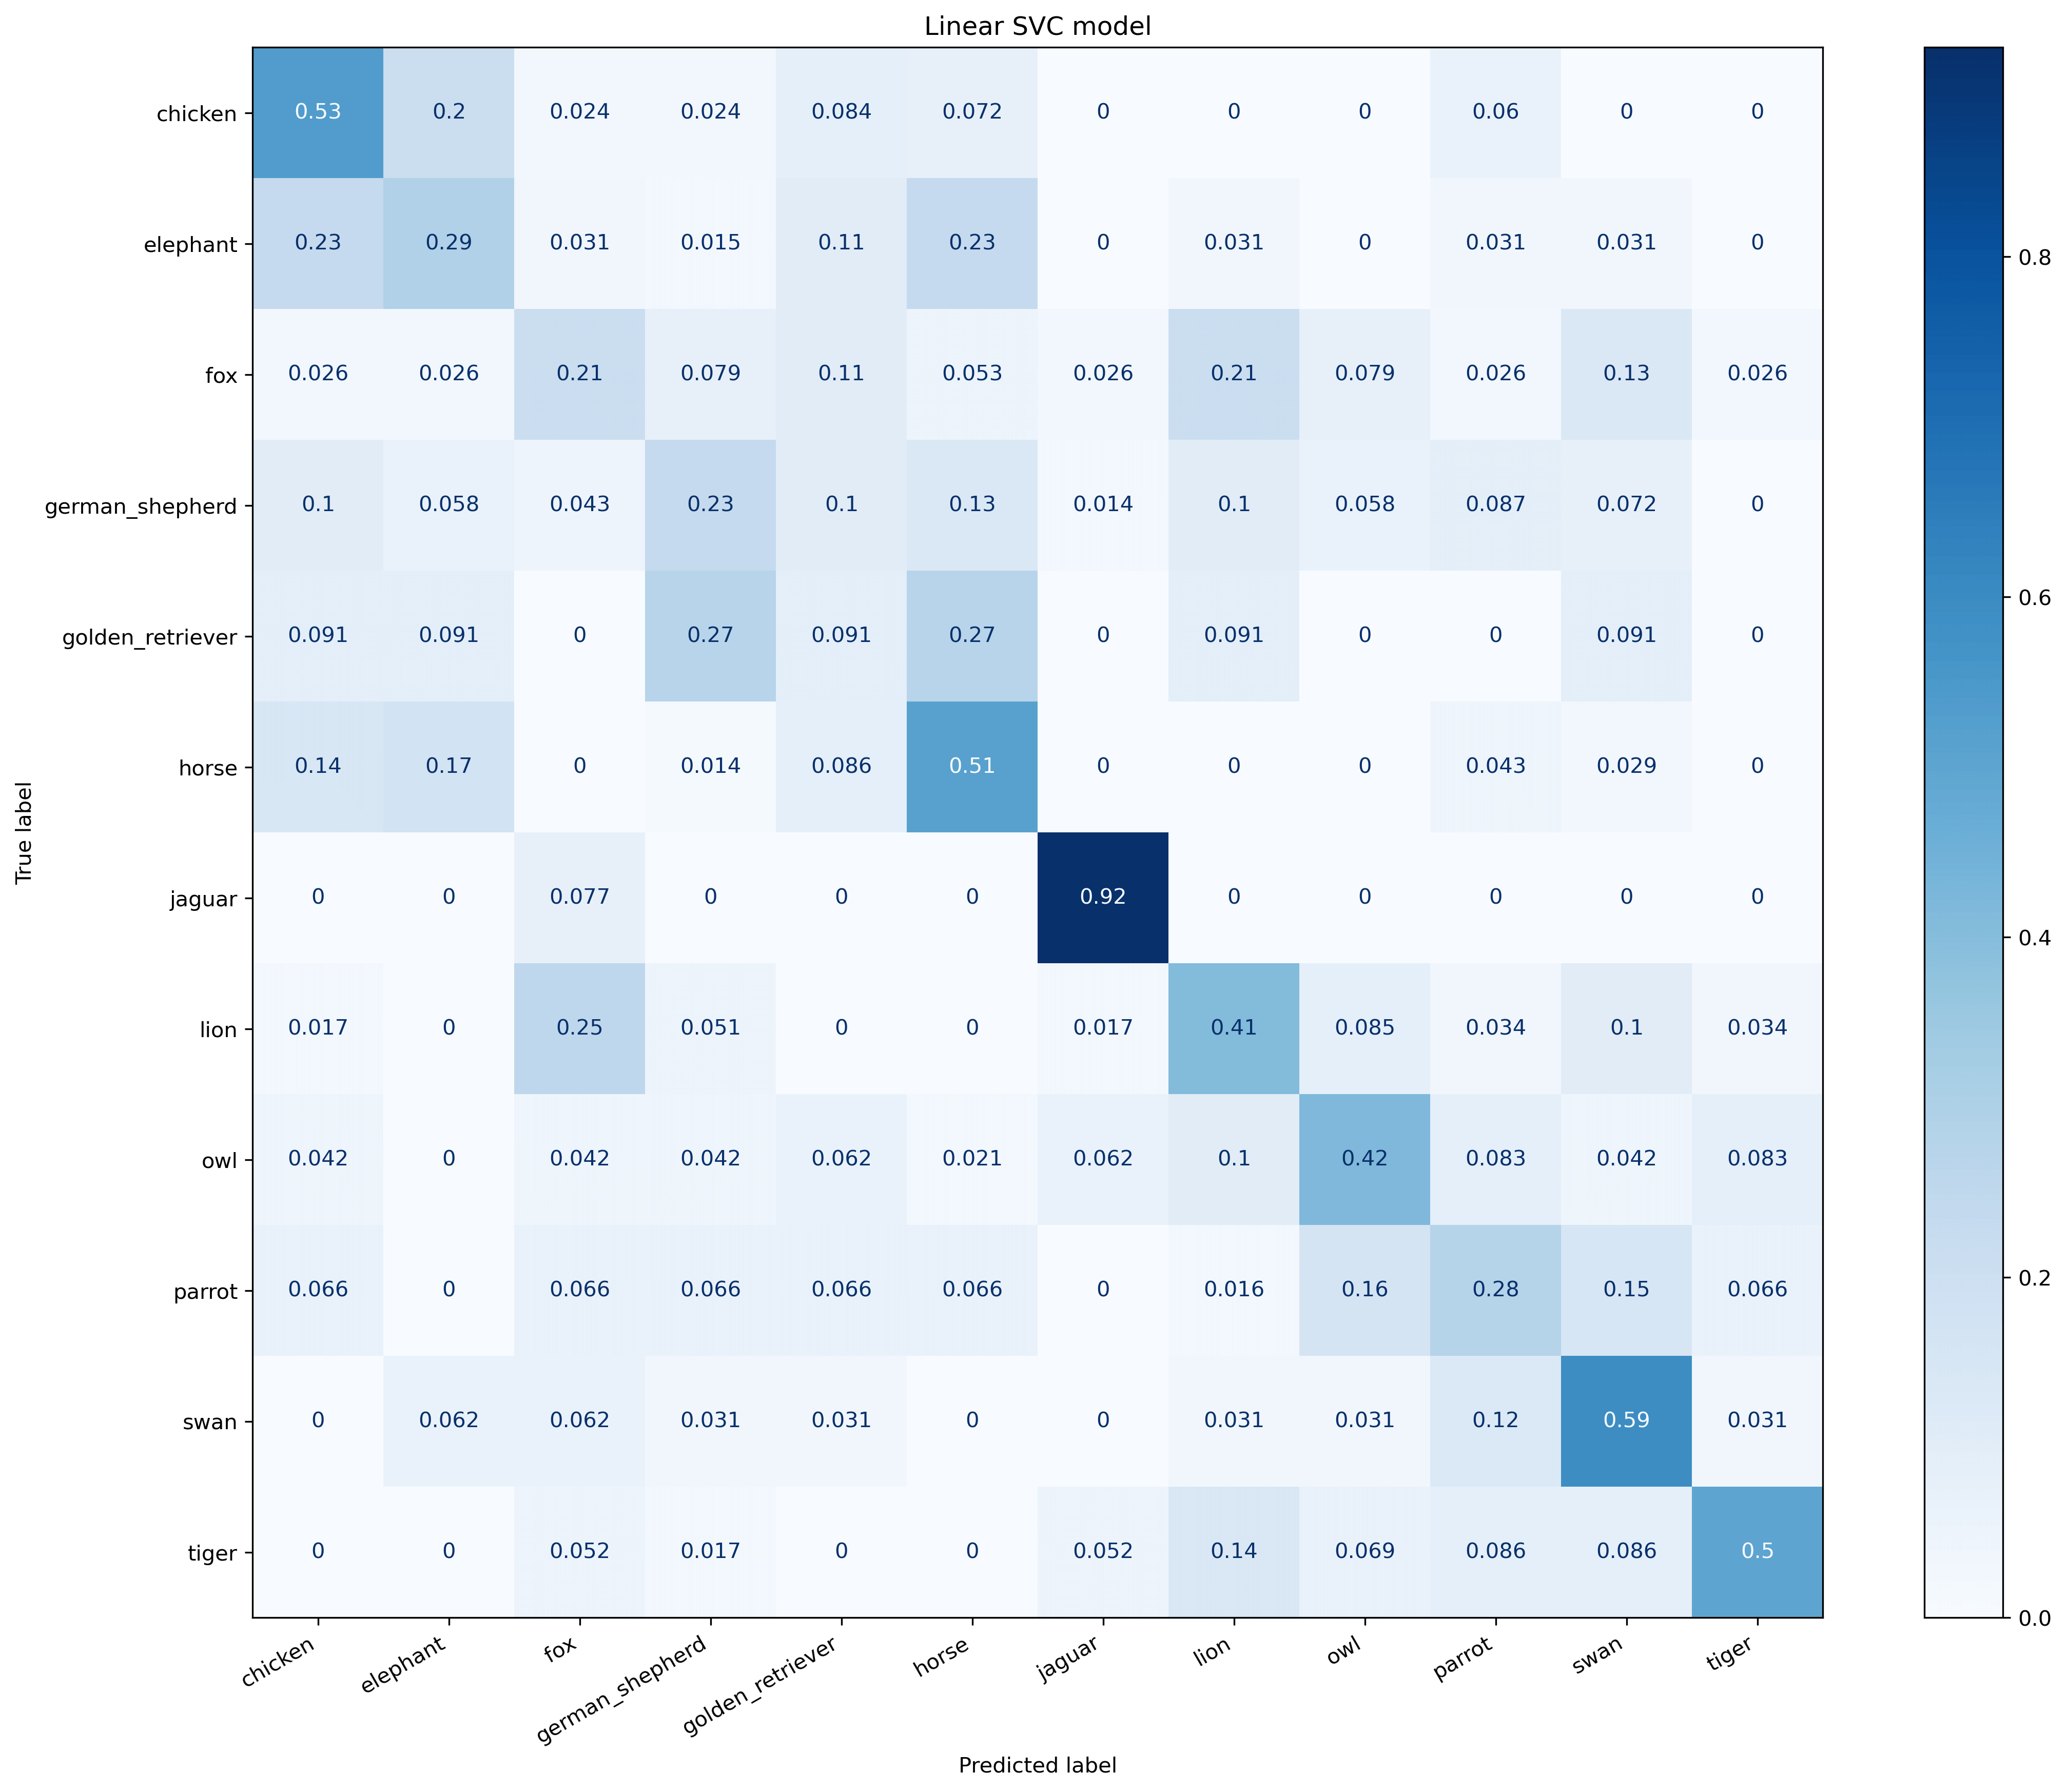
\includegraphics[width=\textwidth]{images/MA/MA_linSVC_normalised.png}}
        \captionsetup{width=0.9\linewidth}
        \captionsetup{justification=centering}
        \caption{Normalised CM.}
    \end{subfigure}
    \captionsetup{width=0.9\linewidth}
    \captionsetup{justification=centering}
    \caption{Confusion matrices for the linear Support Vector Classifier model.}
    \label{fig:ma_linsvc_cm}
\end{figure*}